\documentclass[12pt,twocolumn,a4paper]{article}

% ---------------------------------------------------------------
% Page geometry — matches the Guideline: A4, 0.5 inch margins
% ---------------------------------------------------------------
\usepackage[
  a4paper,
  top=0.5in,
  bottom=0.5in,
  left=0.5in,
  right=0.5in,
  columnsep=0.25in
]{geometry}

% ---------------------------------------------------------------
% Core packages
% ---------------------------------------------------------------
\usepackage{times}
\usepackage{amsmath,amssymb,amsthm}
\usepackage{booktabs}
\usepackage{graphicx}
\usepackage{microtype}
\usepackage{fancyhdr}
\usepackage{titlesec}
\usepackage{hyperref}
\usepackage{listings}
\usepackage{tikz}
\usetikzlibrary{positioning,arrows.meta}

% Citation styling (Strictly Numbers)
\usepackage[numbers,sort&compress]{natbib}
\setlength{\bibsep}{0.4ex plus 0.1ex minus 0.1ex}

\hypersetup{
    colorlinks=true,
    linkcolor=blue,
    filecolor=magenta,
    urlcolor=blue,
    citecolor=blue,
}

% Algorithm packages
\usepackage{algorithm}
\let\algorithmic\relax
\let\endalgorithmic\relax
\usepackage{algpseudocode}

\usepackage[table]{xcolor}
\usepackage{eurosym}
\usepackage{setspace}
\usepackage{placeins} % Retained to support \FloatBarrier at the end

% Math and theorem packages
\theoremstyle{plain}
\newtheorem{theorem}{Theorem}[section]
\newtheorem{proposition}[theorem]{Proposition}
\newtheorem{lemma}[theorem]{Lemma}
\newtheorem{corollary}[theorem]{Corollary}
\theoremstyle{definition}
\newtheorem{definition}[theorem]{Definition}
\newtheorem{assumption}[theorem]{Assumption}
\theoremstyle{remark}
\newtheorem{remark}[theorem]{Remark}

% Custom macros
\newcommand{\train}{\mathcal{D}_{\mathrm{tr}}}
\newcommand{\test}{\mathcal{D}_{\mathrm{te}}}
\newcommand{\R}{\mathbb{R}}

% ---------------------------------------------------------------
% Font sizes & spacing
% ---------------------------------------------------------------
\setlength{\parskip}{0pt}
\setlength{\parindent}{0pt}
\linespread{1.0}

% ---------------------------------------------------------------
% Section heading styles
% ---------------------------------------------------------------
\titleformat{\section}
  {\normalfont\fontsize{12}{14}\bfseries\raggedright}
  {\thesection.}{0.5em}{}
\titlespacing{\section}{0pt}{6pt}{3pt}

\titleformat{\subsection}
  {\normalfont\fontsize{11}{13}\bfseries\raggedright}
  {\thesubsection.}{0.5em}{}
\titlespacing{\subsection}{0pt}{5pt}{2pt}

% ---------------------------------------------------------------
% Running head (Updated to exactly match the Title)
% ---------------------------------------------------------------
\pagestyle{fancy}
\fancyhf{}
\renewcommand{\headrulewidth}{0.4pt}
% Shrunk slightly to 9pt so the very long title fits on one line
\fancyhead[C]{\fontsize{9}{11}\selectfont\textbf{A Multi-Output Surrogate Modeling Framework for Scenario-Based Maritime and Border Logistics Under Brexit Constraints}}
\fancyfoot[C]{\thepage}
\fancypagestyle{plain}{\fancyhf{}\fancyfoot[C]{\thepage}}

% ---------------------------------------------------------------
% Title block
% ---------------------------------------------------------------
\makeatletter
\renewcommand{\maketitle}{%
  \twocolumn[{%
    \vspace*{-0.5em}
    \hrule height 1pt
    \vskip 6pt
    {\centering\fontsize{16}{18}\bfseries\selectfont \@title \par}
    \vskip 6pt
    \hrule height 1pt
    \vskip 10pt
    {\centering\fontsize{12}{14}\selectfont \@author \par}
    \vskip 14pt
  }]%
}
\makeatother

\title{A Multi-Output Surrogate Modeling Framework for Scenario-Based Maritime and Border Logistics Under Brexit Constraints}

\author{%
  \textbf{Sakshi Dhamane} \quad
  \textbf{Iniyanila Gnanasekar} \quad
  \textbf{Uthara Prarath}\\[4pt]
  \fontsize{11}{13}\selectfont
  Maynooth University, Kildare, Ireland \\[2pt]
}

% ---------------------------------------------------------------
\begin{document}
% ---------------------------------------------------------------

\maketitle
\thispagestyle{plain}

% ---------------------------------------------------------------
\section*{Abstract}
% ---------------------------------------------------------------
We present a practical human-interactive machine learning framework for scenario-based prediction in cross-border logistics systems, targeting post-Brexit implications on the Irish agri-food exports in Ireland-GB-EU freight operations.AnyLogic Cloud simulation supports credible what-if analysis but imposes high adoption friction (${\sim}$157 parameters, ${\sim}$EUR\,2{,}520 annual API subscription) for non-expert managers. We learn \emph{surrogate regressors}  nearly orthogonal Latin hypercube design (NOLHC) dataset having correlations between the columns in the design matrix that are in the interval of (-0.3, 0.3),  The design maps ($n{=}129$, $d{=}35$, $K{=}20$) and deploy a human-on-the-loop \emph{Decision Intelligence} web UI with millisecond inference. To handle heterogeneous output behavior under small-sample conditions (129 design rows), we perform per-target model selection across a diverse candidate set including linear, kernel, tree-based, and boosting regressors. The pipeline uses an 80/20 train-hold-out split, repeated 10-fold CV on the training pool only, paired $t$-tests and Friedman/Nemenyi diagnostics across 19 model families, SHAP explainability before final sign-off, and conformal-style uncertainty bands. We integrate SHAP-based attribution for model-level interpretability and expose the full stack in an interactive decision interface that supports route and border-policy interventions with conformal prediction range. Hold-out validation improves over mean/OLS baselines on 19/20 targets (exception: \texttt{Waiting Time Inbound Non Agri Rosslare}, $-0.6\%$), with largest gains on agri transit-time KPIs (${\sim}$74--79\% RMSE reduction)$R^2=0.821$ (mean $R^2=0.735$), with strong performance on most targets and clear diagnostics on failure cases.We discuss small-$n$ extrapolation risk, non-causal SHAP, and governance constraints for  port-stakeholder review. The result is a transparent, deployment-ready surrogate modelling pipeline for policy stress-testing in freight systems with limited labelled data.

% ---------------------------------------------------------------
\section{Introduction}
% ---------------------------------------------------------------
Brexit shifted Irish agri-food logistics from barrier-free movement to a high-intervention border regime with mandatory customs and SPS protocols, increasing delivery times and administrative burden \cite{mahfouz2019,mahfouz2020}.When the UK landbridge incurs delays and border friction, operators redirect capacity to direct maritime corridors (e.g.\ Rosslare--Cherbourg), changing the feasible set of route and staffing policies \cite{copenhagen2018,ivanov2025}.Stakeholders must evaluate post-Brexit models under varying border-control and staffing assumptions at Dublin and Rosslare---comparing landbridge vs.\ direct EU routes while tracking KPIs (transit times, waiting times, customs/DAFM utilisation, queue lengths).Agent-based simulation (AnyLogic) remains the ground-truth engine but is ill-suited to iterative workshops: the cloud model exposes ${\sim}$157 inputs, and API access carries substantial subscription cost; practitioners without deep simulation expertise struggle to set inspection rates and resource allocations \cite{byrne2009,amroune2019}.Initially we tried to adopt the dataset from the AnyLogic simulation runs; by analysing the dataset, many of the parameters are zero-inflated values because the simulation is scenario-based. To overcome this We propose an ML-driven web UI trained on NOLHC simulation runs \cite{cioppa2007,viana2016,bogoclu2021}, delivering near real-time KPI prediction with reduced parameter complexity.
The system follows a \emph{human-on-the-loop} protocol: surrogates accelerate ``if-then'' exploration while domain experts retain authority over scenario assumptions and metric interpretation.

\paragraph{Prototype expectations.}
The delivered prototype must (i) visualise simulation outcomes for non-experts, (ii) provide hold-out-validated surrogates per KPI, (iii) quantify uncertainty via interval outputs, and (iv) communicate drivers via SHAP and persona-based attribution in the UI decision layer.

A credible artifact additionally requires:
(i) rigorous model comparison and held-out evaluation,
(ii) explainability tied to the selected model per output,
(iii) scenario governance preventing implausible inputs, and
(iv) reproducible packaging for independent review.

This setting has three key challenges: (i) multi-output heterogeneity (20 targets with distinct noise scales and dynamics), (ii) low-data regime ($n=129$), and (iii) need for interpretable and uncertainty-aware outputs suitable for operational decision support.

\begin{itemize}
 \item We formulate multi-output post-Brexit RoRo logistics prediction as supervised learning surrogate model from a 129-run NOLHC design with explicit output-domain constraints at deployment. 
 \item We implement an end-to-end experimental protocol: repeated CV on the training pool only, paired $t$-tests on matched fold errors, mentor-requested Friedman/Nemenyi diagnostics, pre-conformal checkpoints, SHAP before final hold-out sign-off, and composite model selection for reporting  \cite{vovk2005algorithmic,angelopoulos2021gentle}, and explainability for governance using SHAP attribution layer\cite{lundberg2017shap}.
 \item We deliver an integrated \textbf{human-facing decision intelligence} web UI with scenario policy locks, real-time inference, SHAP driver panels with per-target selection across all 20 outputs, and reliability guardrails (clipping, input realism checks).
\end{itemize}

% ---------------------------------------------------------------
\section{Problem Formulation}
\label{sec:Problem}
% ---------------------------------------------------------------
Let $x \in \mathbb{R}^{35}$ denote logistics and border-operation inputs (trade volumes, route capacities, check durations, staffing, and inspection proportions). Let $y \in \mathbb{R}^{20}$ denote output KPIs (transport times, waiting times, and utilization fractions).

\subsection{Problem Setup}
We model post-Brexit freight-system behavior as a multi-output supervised regression task. Let $x \in \mathbb{R}^{35}$ denote operational inputs (trade volumes, route allocations, capacities, check durations, staffing, and inspection proportions), and let $y \in \mathbb{R}^{20}$ denote target KPIs (transport times, waiting times, and resource utilization). We train one predictor per target,
\[
f_t: \mathbb{R}^{35}\rightarrow \mathbb{R},\quad t=1,\dots,20,
\]
with target-specific model class and hyperparameters selected from a shared candidate pool. Inference returns point predictions, uncertainty intervals, and scenario deltas versus baseline.

\paragraph{Inputs.}
Features include trade volumes (tonnes), landbridge/direct route volumes, vessel capacities, check times, resource counts (customs sheds, DAFM bays), and route-mix fractions (green/red/pre-boarding shares).

\paragraph{Outputs.}
Targets span agri/non-agri waiting and transit times, landbridge and direct-route performance, and customs/DAFM utilisation at Dublin and Rosslare (see project crosswalk tables).

\subsection{Surrogate modeling objective}
We consider a simulation-generated dataset of $n$ design points with input vector
$\mathbf{x}_i \in \mathbb{R}^{d}$ and multi-target output vector $\mathbf{y}_i \in \mathbb{R}^{K}$ for $i=1,\ldots,n$.
Each coordinate $y_{i,k}$ corresponds to a continuous operational KPI (e.g., transit time, waiting time, utilisation).

For each target $k \in \{1,\ldots,K\}$, we learn a predictor
$f_k : \mathbb{R}^{d} \rightarrow \mathbb{R}$ from training data $\{(\mathbf{x}_i, y_{i,k})\}_{i \in \mathcal{I}_{\mathrm{tr}}}$
that minimises out-of-sample error under cross-validation, selecting both model class and hyperparameters.
Let $\hat{y}_{i,k} = f_k(\mathbf{x}_i)$ denote predictions on held-out points $i \in \mathcal{I}_{\mathrm{te}}$.

\subsection{Candidate Model Family and Hyperparameter Search}
For small-sample, simulation-based design by using nearly orthogonal LHS, implementing a set of surrogate models is justified because no single algorithm is uniformly best and different methods trade off bias, variance, smoothness, and uncertainty quantification. For each target, we evaluate a diverse candidate family including tree ensembles, linear regularized models, kernel methods, and boosting distinguish them Random Forest \cite{breiman2001random}, Gradient Boosting \cite{friedman2001gradient}, XGBoost \cite{chen2016xgboost}, LightGBM \cite{ke2017lightgbm}, CatBoost \cite{prokhorenkova2018catboost}, Gaussian Processes \cite{rasmussen2006gpml}, SVR \cite{cortes1995svm}, Ridge \cite{hoerl1970ridge}, Lasso \cite{tibshirani1996lasso}, and ElasticNet \cite{zou2005elasticnet}, along with baseline regressors. Hyperparameters are selected by cross-validation (CV) RMSE minimization on the training split.

To improve reliability under small-$n$ conditions, the implementation supports repeated CV (default repeated 10-fold in the pipeline scripts), and records fold-wise RMSE distributions for downstream statistical comparison.

\paragraph{Domain constraints at deployment.}
Let $\Pi_k$ denote projection to feasible ranges (e.g.\ non-negative times, utilisation in $[0,1]$).
Deployed predictions are $\tilde{y}_{i,k} = \Pi_k(f_k(\mathbf{x}_i))$, with UI indication when clipping occurs.

\begin{table*}[t]
\centering
\footnotesize
\setlength{\tabcolsep}{5pt}
\renewcommand{\arraystretch}{1.2}
\caption{Regression models and key strengths for LHS surrogates.}
\label{tab:model_families}
\begin{tabular}{|>{\columncolor{blue!15}}p{2.4cm}|p{4.6cm}|p{4.8cm}|}
\hline
\rowcolor{blue!22}
\textbf{Family} & \textbf{Key strength for LHS surrogates} & \textbf{Literature review evidence} \\
\hline
GP (RBF/Mat\'ern) &
Smooth interpolation + uncertainty, small number of samples &
(Marrel and Iooss, 2024; Bogoclu et al., 2021 \cite{marrel2024}) \\
\hline
SVR-RBF/Poly &
Nonlinear small-sample modeling, kernel flexibility &
(Yalsavar et al., 2022; Mienye and Sun, 2022) \cite{yalsavar2022} \\
\hline
Gradient boosting &
State of the Art (SOTA) tabular accuracy, complex interactions &
(Tay, Narasimhan and Hastie, 2021; Jolicoeur-Martineau et al., 2023)\cite{tay2021}\\
\hline
RF / ExtraTrees &
Strong, robust baselines, low tuning cost &
(Bent\'ejac et al., 2019; Marrel and Iooss, 2024)\cite{bentejac2019} \\
\hline
Polynomial + linear regs &
Interpretability; strong when surface near-polynomial/linear &
(Friedman, Hastie and Tibshirani, 2010)\cite{friedman2001gradient} \\
\hline
KNN / MLP / AdaBoost &
Local structure, DL baseline, classic boosting &
(Halder et al., 2024; Shams et al., 2024)\cite{halder2024} \\
\hline
\end{tabular}
\end{table*}

\subsection{Statistical Model Comparison and Selection}
Beyond selecting by mean CV RMSE alone, we perform pairwise model comparisons using fold-wise paired testing \cite{student1908probable,dietterich1998approximate}. For each target, these comparisons are aggregated into model-selection policies (CV-only and composite score variants). This allows robust per-target specialization instead of enforcing a single global model family across all outputs.

\subsection{Uncertainty Quantification}
After selecting and evaluating target models on hold-out data, we construct residual-quantile predictive intervals:
\[
[\hat{y}-q_\alpha,\hat{y}+q_\alpha], \quad q_\alpha=\mathrm{Quantile}_\alpha(|y-\hat{y}|).
\]
Coverage levels are adaptively chosen from \{0.90, 0.95, 0.99\} according to relative model error, yielding descriptive conformal-style uncertainty summaries \cite{vovk2005algorithmic,angelopoulos2021gentle} for deployment-facing interpretation.

\subsection{Explainability Layer}
For each selected target-model pair, we compute SHAP attributions \cite{lundberg2017shap}. Tree-based explainers are used where supported; otherwise model-agnostic explainers with background masking are applied. We report global mean-$|\mathrm{SHAP}|$ rankings and local diagnostic plots to identify influential operational factors.

\subsection{Scenario-to-Feature Inference Mapping}
The deployed inference layer transforms scenario controls into feature vectors through rule-based mappings (route family and border family), bounded clipping, and dynamic parameter overrides. This enables real-time scenario simulation while preserving feature-domain constraints required by trained surrogate models.

\section{Related Work}
\label{sec:related}

\paragraph{Post-Brexit logistics simulation.}
Simulation is essential in supply chain analysis because it enables the modelling of uncertainty and complex system interactions that approaches cannot capture effectively. By replicating stochastic behaviours, such as demand variability, transport delays, and regulatory changes, it allows decision-makers to test scenarios and evaluate outcomes without real-world risk. This is particularly important in contexts like Brexit, where simultaneous disruptions across trade flows, border procedures, and transport routes create great uncertainty. As simulation provides a robust framework for scenario analysis, strategic planning, and resilience assessment in supply chain systems.\citet{Ivanov2021}.\citet{mahfouz2019} and \citet{mahfouz2020} model post-Brexit agri-fresh and Irish freight corridors; \citet{copenhagen2018} quantify trade-route shifts away from the UK landbridge.
Agent-based and hybrid simulation remain the credibility layer for border and port KPIs \citep{ivanov2025,byrne2009,amroune2019}.

\paragraph{Machine Learning Surrogate Modelling}
By training machine learning models on a representative set of simulation outputs, surrogates can approximate system behaviour and generate predictions much faster, enabling efficient scenario testing without repeatedly executing expensive simulations. Using the NOLHC data, this approach improved scalability and reduced costs compared to running the full AnyLogic model across a large design space. However, this efficiency comes with a trade-off in accuracy, as surrogate performance depends on the quality and coverage of the training data derived from the original simulation. Gaussian-process emulators and design-based metamodels are standard for expensive simulators 

\paragraph{Model Choices for NOLHC Surrogate Modelling}
Nearly orthogonal Latin hypercube designs improve space-filling coverage at modest run budgets \citep{cioppa2007,viana2016,bogoclu2021}.
Surrogate reviews emphasise bias--variance trade-offs, extrapolation risk, and validation discipline when $n$ is small 
Our setting differs in scale ($n{=}129$) and output multiplicity ($K{=}20$), motivating diverse model families rather than a single GP per target.
\item Guassian Process and Kernel SVR: Guassian Process(GP) regression is a standard surrogate for expensive computer experiments providing a probablistic predictive distribution and uncertainity estimates, ideal for sequential design and reliability/uncertainity analysis \citep{marrel2024, bogoclu2021, Cheng2017 }. GP is particularly effective for smooth responses and small to moderate sample sizes. Kernel SVR handles monlinear, high-dimensional problems with small samples, with strong generalization through margin maximization, making it a natural competitor to GP in surrogate-based design \citep{Cheng2017}.Specialized kernels (e.g., orthogonal polynomials, universal kernels) improve capture of complex interactions \citep{Ustun2006}

\item Tree Ensembles and Gradient Boosting: Ensemble methods(RF, GBM, XGBoost, LightGBM, CatBoost, AdaBoost) are widely recognised as state of the art on tabular data, combining robustness, nonlinearity modeling and strong average performances across many benchmarks \citep{bentejac2019}. Random forests are robust to high dimensionality and avoid overfitting while remaining strong baselines \citep{marrel2024, Bentejac2024}. Gradient boosting variants often achieve the best generalization in comparative studies with CatBoost/XGBoost/LightGBM frequently leading, especially for heterogenous/tabular datasets \citep{jolicoeur2023, Bentejac2024, mienye2022}. Tree boosting and bagging are strong baselines for tabular metamodels \citep{friedman2001gbm,breiman2001random,bentejac2019,chen2016xgboost,ke2017lightgbm}.
 \paragraph{Why such breadth, 19 Models?}
Comparative works repeatedly stress that performance is data-dependent and advocate evaluating multiple model families rather than assuming single winner \citep{Preethi2025, marrel2024, chen2016xgboost, bogoclu2021}. For deign Optimization and uncertainty analysis, this breadths helps us to:
\item Capture different functional shapes smooth (GP, polynomial), highly nonlinear/interacting (GBDT, RF, MLP, SVR), and local structures (KNN) \citep{marrel2024, Bentejac2024,Cheng2017}
\item Compare interpretable baselines (linear/polynomial/regularized) against black‑box models \citep{Preethi2025, marrel2024}
\item Obtain uncertainty estimates from GP and Bayesian/regularized linear models for UQ and adaptive sampling \citep{Manfredi2024, Jin2020, tay2021,Bedoui2020}

\paragraph{Model comparison.}
We use paired tests on matched CV fold errors and Friedman/Nemenyi-style rankings 
\paragraph{Uncertainty and explainability.}
We report symmetric intervals from residual quantiles with coverage tied to relative test RMSE, building on conformal foundations \citep{vovk2005algorithmic}; we treat these as descriptive on the hold-out set rather than formal split-conformal guarantees.
Global SHAP attributions support governance review without causal claims \citep{lundberg2017shap}.

\paragraph{Human-Centered UI Design}
Human-centred design is critical in supply chain decision support because it ensures that complex analytical outputs are accessible and actionable for end users. By prioritising usability principles (i.e clear feedback, consistency, and error prevention), it reduces cognitive load and enables faster, higher-quality decision-making without requiring deep technical expertise. In tools like the NOLHC system, where metrics such as transit times, queue lengths, and resource utilisation are presented, clear visualisation and intuitive interaction are essential for effective scenario comparison and interpretation. As a result, well-designed interfaces increase user trust and adoption of model-driven insights, making human-centred design a key component of simulation- and surrogate-based systems \citep{viana2016}

\paragraph{Human-in-the-loop decision support.}
Interactive scenario UIs for logistics are common in operations research \cite{breiman2001random}.Human-in-the-loop AI is important in supply chain decision support because it integrates human judgement into model-driven processes, rather than relying solely on automated outputs. This is particularly valuable in complex logistics contexts, where real-world factors, such as political events or unexpected port congestion, cannot be fully captured in model parameters. By allowing users to adjust assumptions, explore anomalies, and override model recommendations, human-in-the-loop approaches improve both decision quality and user confidence. In systems like the ML surrogate tool, user-defined inputs are actively incorporated into the model to generate updated performance indicators, supporting more informed and context-aware decisions.
Our contribution couples \emph{auditable} ML selection artifacts with explainability, persona-based narration, and policy-governed inputs in a human-on-the-loop protocol 

\paragraph{Synthesis & Research Gap.}
The research shows that simulation is essential for modelling uncertainty in supply chains, while machine learning surrogates improve scalability, human-centred design enhances usability, and human-in-the-loop approaches ensure contextual relevance and decision quality. However, these elements are often applied in isolation, with limited integration into a unified decision support framework. This creates a research gap for developing a simulation-based system that combines these approaches to deliver scalable, interpretable, and user-driven supply chain analysis.

% ---------------------------------------------------------------
\section{Dataset characterisation}
\label{sec:Dataset characterisation}
% ---------------------------------------------------------------

The experimental corpus comprises $n{=}129$ complete AnyLogic simulation runs from a \emph{Nearly Orthogonal Latin Hypercube} (NOLHC) design over $d{=}35$ continuous input parameters and $K{=}20$ continuous simulation outputs (KPIs).
Each run maps a joint draw of trade volumes (tonnes), route-mode allocations (landbridge vs.\ direct EU, including Cherbourg shift volumes), vessel capacities (trailers), checkpoint check times (minutes), staffing counts, and border-check route fractions in $[0,1]$, to agri and non-agri transit and wait times (hours), route-level transit and wait KPIs, and customs/DAFM staff utilisation (unitless fractions).
Processed matrices contain no missing values.
Inputs span heterogeneous physical units and magnitudes (e.g.\ trade flows in hundreds of thousands of tonnes vs.\ fractions near unity), motivating per-feature standardisation for distance-based learners while tree ensembles use raw inputs.

Descriptive statistics on all 129 runs show pronounced \emph{scale heterogeneity} among targets: landbridge outbound transit (\texttt{TT\_OB\_LB}) is tightly concentrated (mean ${\approx}25.7$\,h, s.d.\ ${\approx}0.46$\,h on $[25,27]$\,h), whereas inbound landbridge waits and several agri KPIs exhibit much larger dispersion (e.g.\ \texttt{WT\_IB\_LB}: mean ${\approx}61.5$\,h, s.d.\ ${\approx}62.5$\,h).
Eight of twenty outputs have $|\mathrm{skewness}|{>}1$; agri outbound transit (\texttt{TT\_OB\_Agri}, skew ${\approx}3.0$) and non-agri inbound wait at Rosslare (\texttt{WT\_IB\_NA\_Ross}, skew ${\approx}7.5$) are strongly right-skewed, indicating a minority of design points with unusually long delays.
Utilisation KPIs are bounded near $[0,1]$ with smaller variance (e.g.\ \texttt{Uti\_Cus\_D} mean ${\approx}0.90$, s.d.\ ${\approx}0.14$).
Pairwise correlations among outputs are moderate on average (mean $|r|{\approx}0.30$) but several KPI pairs exceed $|r|{=}0.7$, reflecting shared congestion dynamics across routes and commodities; surrogates are therefore trained as \emph{multi-output regressors} (one model per KPI) rather than as a single joint classifier.

For model development, indices are permuted with seed 42 and partitioned into a training pool of $|\train|{=}103$ (${\approx}80\%$) and a hold-out set of $|\test|{=}26$ (${\approx}20\%$); the hold-out rows are excluded from cross-validation, hyperparameter search, and scaler fitting.
The small design size and non-uniform output scales favour flexible regressors (ensembles, Gaussian processes) alongside linear baselines, and caution against extrapolation beyond the NOLHC envelope.

\begin{table}[t]
  \centering
  \caption{Variable groups in the NOLHC design (counts).}
  \label{tab:var-groups}
  \small
  % Changed column definitions to p{} to enable text wrapping
  \begin{tabular}{@{} p{0.40\columnwidth} c p{0.45\columnwidth} @{}}
    \toprule
    \multicolumn{3}{@{}l}{\textit{Inputs} ($d{=}35$)} \\
    \midrule
    Group & \# & Examples \\
    \midrule
    Trade volume shifts & 4 & Non-agri/agri import--export totals \\
    Direct vs.\ land-bridge routing & 8 & Cherbourg shifts; LB/DR splits \\
    Land-bridge corridor volumes & 4 & Mode-specific tonne flows \\
    Vessel capacity (IRE--GB) & 5 & Dublin/Rosslare route capacities \\
    Customs expertise \& resources & 6 & Check times; shed/bay counts \\
    Border-check interventions & 8 & Green/red/pre-board fractions \\
    \midrule
    \multicolumn{3}{@{}l}{\textit{Outputs} ($K{=}20$)} \\
    \midrule
    Agri transit \& wait & 6 & \texttt{TT\_OB\_Agri}, \texttt{WT\_IB\_A\_*} \\
    Non-agri wait & 4 & \texttt{WT\_IB\_NA\_*}, \texttt{WT\_OB\_NA\_*} \\
    Route transit \& wait & 6 & Landbridge/direct \texttt{TT\_*}, \texttt{WT\_*} \\
    Staff utilisation & 4 & \texttt{Uti\_Cus\_*}, \texttt{Uti\_DAFM\_*} \\
    \bottomrule
  \end{tabular}
\end{table}
% -----------------------------------------------------------------------------
\section{Method}
\label{sec:method}

We learn \emph{multi-output surrogates} mapping simulator inputs to logistics KPIs with auditable model choice and millisecond inference.
Design and variable groups are in \S\ref{sec:experiments} (Appendix~\ref{app:supp}); dataset counts are omitted here.
For each target $k$, we estimate $f_k$ on $\train$, rank families by repeated CV and nonparametric tests, explain the pre-test composite winner with SHAP, and deploy $(f_1,\ldots,f_K)$ with projection $\Pi_k$ and uncertainty bands.
A single reproducible run fits scalers, logs fold-wise RMSE, exports \texttt{.joblib} artefacts, and feeds the Decision Intelligence UI.
Figure~\ref{fig:pipeline} and Algorithm~\ref{alg:cv-target} (Appendix~\ref{app:workflow}) summarise the workflow.

\subsection{Problem formulation and I/O}
\label{sec:method-io}

The \emph{input} is design matrix $\mathbf{X} \in \R^{n \times d}$ with rows $\mathbf{x}_i \in \R^d$ and multi-target matrix $\mathbf{Y} \in \R^{n \times K}$ with entries $y_{i,k}$.
For target $k$, we extract $\mathbf{y}^{(k)} = (y_{1,k},\ldots,y_{n,k})^\top$ and fit learner $f_k(\cdot;\theta)$ from family $m \in \mathcal{M}$ with hyperparameters $\theta \in \mathcal{G}_m$, predicting $\hat{y}_{i,k} = f_k(\mathbf{x}_i;\theta)$ on held-out indices.
At deployment, scenario $\mathbf{x}_\star$ yields $\tilde{y}_{\star,k} = \Pi_k(f_k(\mathbf{x}_\star))$ where $\Pi_k$ clips or bounds predictions to simulator-feasible ranges (\S\ref{sec:setup}).
We fit \emph{one surrogate per KPI} rather than a joint vector regressor: each $f_k$ is selected and tuned independently while sharing $\mathbf{X}$, which avoids forcing a single hypothesis class across heterogeneous targets (transit hours vs.\ unitless utilisation) and isolates failure modes to one KPI.
The multi-output map is therefore a tuple $(f_1,\ldots,f_K)$ of regressors, not a single shared representation layer.
Crosswalks map feature indices to domain labels for SHAP and the UI without altering $\mathbf{X}$.
On validation $\mathcal{V}$, $\mathrm{RMSE}_k = \sqrt{|\mathcal{V}|^{-1}\sum_{i \in \mathcal{V}} (y_{i,k} - \hat{y}_{i,k})^2}$ is the primary tuning objective; MAE and $R^2$ on $\test$ complement RMSE for skewed wait-time KPIs.
Hyperparameter search minimises mean CV RMSE across $30$ fold scores, tie-breaking on lower fold-wise RMSE standard deviation when means tie.

\subsection{Training protocol and hyperparameter search}
\label{sec:method-protocol}

Indices are permuted once (\texttt{random\_state=42}; \texttt{split\_meta.json}) into $\train$ and $\test$ (sizes in Appendix~\ref{app:supp}).
$\test$ is excluded from CV, \texttt{ParameterGrid} search, scaler fitting, Friedman/Nemenyi blocks, and \texttt{composite\_pre\_test}; it is used only for final metrics and interval calibration (\S\ref{sec:experiments}).
All $d$ parameters enter as numeric features without PCA.
\texttt{StandardScaler} is fit on $\mathbf{X}_{\train}$ for GPR, SVR, polynomial--Ridge, penalised linear models, KNN, MLP, and \texttt{Baseline\_OLS}; trees and CatBoost use raw $\mathbf{x}$.
\textbf{Repeated 10-fold CV} on $\train$ uses \texttt{RepeatedKFold} with three repeats ($30$ RMSE values per configuration); every $\theta \in \mathcal{G}_m$ is evaluated for each $(k,m)$.
The winning configuration minimises mean CV RMSE with the stability tie-break above.
Aligned fold-wise errors support paired $t$-tests and are logged in \texttt{cv\_fold\_details.xlsx} (Algorithm~\ref{alg:cv-target}).

\subsection{Surrogate learners}
\label{sec:method-learners}

\texttt{Baseline\_Mean} predicts the training mean; \texttt{Baseline\_OLS} is least squares on scaled features---both optional in paired checks, excluded from Friedman blocks over $\mathcal{M}$ ($|\mathcal{M}|{=}19$).
Each core family has a \texttt{ParameterGrid} in \texttt{models.py} and is trained for every $k$:
\texttt{GPR\_RBF}, \texttt{GPR\_Matern}, \texttt{RandomForest}, \texttt{ExtraTrees}, \texttt{GradientBoosting}, \texttt{AdaBoost}, \texttt{XGBoost}, \texttt{LightGBM}, \texttt{CatBoost}, \texttt{SVR\_RBF}, \texttt{SVR\_Poly}, \texttt{PolynomialReg\_deg2}, \texttt{PolynomialReg\_deg3}, \texttt{Ridge}, \texttt{Lasso}, \texttt{ElasticNet}, \texttt{BayesianRidge}, \texttt{KNN}, and \texttt{MLP}.

\emph{Scaled linear and polynomial family.}
\texttt{Ridge}, \texttt{Lasso}, and \texttt{ElasticNet} penalise $\|\boldsymbol{\beta}\|_2^2$, $\|\boldsymbol{\beta}\|_1$, or both with log-spaced $\alpha$ (and $\ell_1$ ratio for elastic net).
\texttt{BayesianRidge} uses Gaussian coefficient priors; \texttt{PolynomialReg\_deg2/deg3} use \texttt{PolynomialFeatures} plus \texttt{Ridge} (often strong on wait-time KPIs; \S\ref{sec:experiments}).

\emph{Tree ensembles and gradient boosting.}
\texttt{RandomForest} and \texttt{ExtraTrees} bag depth-limited trees \citep{breiman2001random}; \texttt{GradientBoosting}, \texttt{AdaBoost}, \texttt{XGBoost}, and \texttt{LightGBM} add stage-wise boosting \citep{friedman2001gbm,chen2016xgboost,ke2017lightgbm}.
All use raw $\mathbf{x}$ and frequently lead CV for transit-time targets (\S\ref{sec:experiments}).

\emph{Kernel, neighbourhood, and neural surrogates.}
\texttt{SVR\_RBF} and \texttt{SVR\_Poly} implement $\epsilon$-insensitive RKHS regression with grids over $C$, $\epsilon$, and kernel hyperparameters on scaled inputs.
\texttt{KNN} averages $k \in \{3,5,7,10,15\}$ neighbours with uniform or distance weights and $L_1/L_2$ metrics.
\texttt{MLP} uses one--two hidden layers (50--100 units), ReLU activations, and $\ell_2$ weight decay; KNN and MLP diversify rankings but seldom win composite selection on thin designs.
All nineteen families share identical folds, logging, and selection logic so differences reflect inductive bias rather than protocol drift.

\texttt{GPR\_RBF} and \texttt{GPR\_Matern} posit $f \sim \mathcal{GP}(0,k)$ with
$k(\mathbf{x},\mathbf{x}') = \sigma_f^2 C \cdot k_{\mathrm{base}}(\mathbf{x},\mathbf{x}') + \sigma_n^2 \delta_{\mathbf{x}\mathbf{x}'}$,
where $k_{\mathrm{base}}$ is RBF or Mat\'ern $\nu{=}1.5$ plus \texttt{WhiteKernel} \citep{santner2003design,forrester2008}; length scales use \texttt{n\_restarts\_optimizer=2} and jitter $\alpha \in \{10^{-10},10^{-6},10^{-3}\}$.
With \texttt{normalize\_y=True}, posterior mean
$\hat{y}_\star = \mathbf{k}_\star^\top (\mathbf{K}+\alpha\mathbf{I})^{-1}\mathbf{y}_{\train}$
yields smooth interpolants well suited to low-noise utilisation surfaces where \texttt{GPR\_Matern} often wins (\S\ref{sec:experiments}); Mat\'ern $\nu{=}1.5$ is less brittle than RBF at short length scales.
Fitting costs $\mathcal{O}(|\train|^3)$ per target, which remains feasible for our training-pool size; we use conformal residuals rather than GPR variance for comparable intervals across families.

\texttt{CatBoost} \citep{bentejac2019} uses \emph{ordered} boosting (gradients for row $i$ use only prior rows in a permutation) and \emph{symmetric} trees (one split predicate per depth), reducing small-$n$ shift when $|\train| \ll 2^d$.
We tune \texttt{iterations}, \texttt{learning\_rate}, and \texttt{depth} $\in \{4,6\}$ with \texttt{random\_seed=42}.
CatBoost and other boosters consume raw numeric features without one-hot encoding in this fully continuous design.

\subsection{Model comparison, explainability, and deployment}
\label{sec:method-compare}

Paired $t$-tests (\texttt{scipy.stats.ttest\_rel}, $\alpha{=}0.05$) on aligned fold RMSEs yield $171$ unordered pairs per target among core families; wins feed composite reporting (40\% CV RMSE, 40\% test RMSE, 20\% win rate) but are descriptive under multiple testing.
\texttt{composite\_pre\_test} (CV + wins only) governs SHAP and pre-conformal steps before $\test$ sign-off, ensuring explainability and interval widths never peek at the hold-out set.

\paragraph{Friedman and Nemenyi.}
Each CV fold is a block; matrix $\mathbf{E} \in \R^{N_{\mathrm{fold}} \times |\mathcal{M}|}$ stores validation RMSEs ($N_{\mathrm{fold}}{=}30$) \citep{demvsar2006statistical,nemenyi1963distribution,jia2025pairwise}.
Friedman tests equal mean ranks; Nemenyi post-hoc uses critical difference
$\mathrm{CD} = q_\alpha \sqrt{|\mathcal{M}|(|\mathcal{M}|+1)/(6N_{\mathrm{fold}})}$ for tier-1 clusters and critical-difference diagrams (Step~2).
Hold-out RMSE (one value per model) is excluded from these blocks.
Step~3 may calibrate top-three CV models on out-of-fold residuals; Step~6 retrains $(m^\star_k,\theta^\star_k)$ on $\train$ before $\test$ evaluation (\S\ref{sec:experiments}).

\paragraph{SHAP.}
For each \texttt{composite\_pre\_test} winner, SHAP values \citep{lundberg2017shap} are computed on $\mathbf{X}_{\train}$ before $\test$ is used.
Trees and CatBoost use \texttt{TreeExplainer}; scaled learners use \texttt{shap.Explainer} with a background masker and scaler-wrapped predict.
Each feature $j$ receives $\phi_{i,j}$ with $\sum_j \phi_{i,j} = \hat{y}_{i,k} - \mathbb{E}[\hat{y}]$; global importance ranks $\mathbb{E}_i[|\phi_{i,j}|]$ via crosswalks (trade, routing, customs, border checks).
SHAP explains model dependence, not causal policy effects (\S\ref{sec:discussion}).

\paragraph{Uncertainty and deployment.}
\label{sec:method-deploy}
Symmetric bands $[\hat{y}_{\star,k} \pm q]$ set $q$ to the $90^{\mathrm{th}}$ percentile of $|\tilde{y}_{i,k}-y_{i,k}|$ on $\test$ (Step~9), reporting empirical vs.\ nominal 90\% coverage; Step~3 may set $q$ from out-of-fold residuals among top-three CV models beforehand.
The scheme follows conformal \emph{ideas} \citep{vovk2005algorithmic,angelopoulos2023conformal,romano2019cqr} but, on a single fixed $\train$/$\test$ partition, does not provide distribution-free guarantees; production deployments should reserve a dedicated calibration fold.
FastAPI (\texttt{POST /api/predict}) serves retrained \texttt{.joblib} models, scalers, interval metadata, and SHAP summaries; the UI groups ${\sim}35$ levers into Volume, Routes, Customs, and Border Checks, applies policy locks, flags $\Pi_k$ clipping, and surfaces error, interval width, CV stability, and SHAP drivers.
Optional LLM personas narrate the same structured snapshot for non-technical mentors.

% -----------------------------------------------------------------------------
\section{Experiments}
\label{sec:experiments}

We evaluate multi-output \emph{regression} surrogates on the NOLHC computer experiment (\S\ref{sec:method}, Figure~\ref{fig:pipeline}).
Table~\ref{tab:data} (Appendix) records 129 design runs, $d{=}35$ inputs, $K{=}20$ KPIs, the 103/26 train--hold-out split, 19 core families, and repeated 10-fold CV ($\times 3$ repeats).
Table~\ref{tab:var-groups} (Appendix) groups trade, routing, capacity, customs, and border-check inputs and the six agri, four non-agri, six route, and four utilisation outputs.
All reported scores are regression errors on continuous hours or utilisation fractions, not classification rates.
The experimental loop mirrors Figure~\ref{fig:pipeline}: fit on $\train$, compare families with repeated CV and paired tests, explain \texttt{composite\_pre\_test} winners with SHAP, then evaluate once on the fixed $\test$ split.

\subsection{Protocol and baselines}
\label{sec:exp-protocol}

We follow \S\ref{sec:method-protocol}: $\test$ is excluded from hyperparameter tuning and \texttt{composite\_pre\_test} SHAP.
Each of 19 core families is scored with \textbf{repeated 10-fold CV} on $\train$ (three repeats, 30 RMSE values per configuration).
\texttt{Baseline\_Mean} and \texttt{Baseline\_OLS} anchor whether the model zoo improves on trivial predictors.

\subsection{Regression metrics and selection}
\label{sec:exp-metrics}

For target $k$ and index set $\mathcal{V}$ (CV or $\test$),
\begin{align}
  \mathrm{RMSE}_k &= \sqrt{\frac{1}{|\mathcal{V}|}\sum_{i\in\mathcal{V}} \bigl(y_{i,k}-\hat{y}_{i,k}\bigr)^2}, \label{eq:rmse}\\
  \mathrm{MAE}_k &= \frac{1}{|\mathcal{V}|}\sum_{i\in\mathcal{V}} \bigl|y_{i,k}-\hat{y}_{i,k}\bigr|, \label{eq:mae}\\
  R^2_k &= 1 - \frac{\sum_{i\in\mathcal{V}}(y_{i,k}-\hat{y}_{i,k})^2}{\sum_{i\in\mathcal{V}}(y_{i,k}-\bar{y}_k)^2}, \label{eq:r2}
\end{align}
with $\bar{y}_k$ the mean of $y_{\cdot,k}$ on $\mathcal{V}$.
RMSE is the primary selection objective; MAE and $R^2$ support interpretation under heavy tails.
Hyperparameter search minimises mean CV RMSE with tie-break on fold RMSE standard deviation.
KPIs are continuous capacity-planning quantities, so we do not binarise them for accuracy, precision, recall, F1, or AUC; doing so would mis-state the port capacity-planning task.
We report \eqref{eq:rmse}--\eqref{eq:r2} plus descriptive interval coverage (\S\ref{sec:results-intervals}).

\textbf{Selection.} Per target $k$, lowest mean CV RMSE across $(m,\theta)$ with $\sigma$ tie-break defines the CV winner (\texttt{cv\_best\_model\_per\_target.csv}).
Aligned fold RMSE vectors support $171$ paired $t$-tests ($\alpha{=}0.05$); win counts inform reporting but are not a multiple-testing guarantee.
Friedman/Nemenyi (Step~2) ranks the 19 core families across 30 repeated-fold blocks and forms tier-1 clusters (Figure~\ref{fig:heatmap-placeholder} in Appendix).
Step~10 composites weight \textbf{40\%} normalised CV RMSE, \textbf{40\%} normalised hold-out RMSE, and \textbf{20\%} paired win rate.
\texttt{composite\_pre\_test} drops the test term for SHAP and pre-conformal checkpoints; Table~\ref{tab:holdout-all} (Appendix) remains the definitive generalisation readout.
Table~\ref{tab:scenarios} (Appendix) lists UI stress families (direct-route shift, non-tariff barriers) for mentor workshops; inference still uses the full 35-parameter vector with policy locks (\S\ref{sec:method-deploy}).

% -----------------------------------------------------------------------------
\section{Results}
\label{sec:results}

\subsection{Cross-validation and hold-out summary}
\label{sec:results-summary}

Table~\ref{tab:holdout-all} (Appendix) summarises hold-out RMSE, MAE, and $R^2$ for representative targets; all 20 appear in \texttt{selected\_holdout\_summary.csv}.
On $\train$, CV-best configurations beat \texttt{Baseline\_Mean} and \texttt{Baseline\_OLS} on mean CV RMSE (\textbf{20/20}).
After retraining on $\train$, hold-out evaluation ($|\test|{=}26$) yields mean test RMSE $5.29$, mean MAE $4.06$, and mean $R^2{=}0.74$.
Deployed surrogates beat the stronger baseline on test RMSE for \textbf{16/20} targets; three wait-time KPIs are within ${\sim}1\%$ of best baseline RMSE while often improving MAE.
Hours-scale transit and wait KPIs dominate the unweighted mean RMSE ($5.29$), so aggregate means should be read alongside per-target tables.
The principal exception is \texttt{WT\_IB\_NA\_Ross} (\texttt{SVR\_RBF}: RMSE $9.65$ vs.\ OLS $9.22$, $+4.7\%$, $R^2{\approx}0.03$).
Largest gains vs.\ OLS are on agri transit: \texttt{TT\_OB\_Agri} (ExtraTrees, $5.41$ vs.\ $26.15$, ${\sim}79\%$, $R^2{=}0.97$) and \texttt{TT\_IB\_Agri} ($7.92$ vs.\ $29.48$, ${\sim}73\%$, $R^2{=}0.97$).

\subsection{Diagnostics, families, and uncertainty}
\label{sec:results-diagnostics}

Figure~\ref{fig:residual-agri} (Appendix) shows tight hold-out fit for \texttt{TT\_OB\_Agri}; Figure~\ref{fig:residual-failure} (Appendix) shows elevated RMSE and bias on \texttt{WT\_IB\_NA\_Ross}; Figure~\ref{fig:residual-util} (Appendix) shows low-error utilisation for \texttt{Uti\_DAFM\_D} ($n{=}26$).
Most targets reach empirical 90\% coverage ${\approx}0.885$; several show heavy tails despite low RMSE.

Tree ensembles (ExtraTrees, CatBoost) dominate skewed agri transit where capacity and trade volumes interact with route mix.
Lasso wins volatile landbridge waits (\texttt{WT\_IB\_LB}, \texttt{TT\_IB\_LB}); GPR\_Matern excels on utilisation (\texttt{Uti\_DAFM\_R} RMSE $0.016$, $R^2{=}0.93$).
For \texttt{WT\_IB\_NA\_Ross}, wide CV $\sigma$ and weak $R^2$ indicate no family consistently beats OLS; deployed SVR trades lower MAE ($2.90$ vs.\ $5.26$) for worse RMSE.
CatBoost wins several direct-route transit targets but can show negative $R^2$ on thin-variance splits (\texttt{TT\_IB\_DR}), reinforcing per-target dashboards in the UI.
Global SHAP on \texttt{composite\_pre\_test} winners ranks \texttt{VCap\_Dub\_*} and agri trade highest for transit; \texttt{ChkTime\_Doc} and DAFM bays lead waits (Figure~\ref{fig:shap-placeholder} in Appendix; \texttt{xai\_shap\_top\_features\_long.csv}).
Friedman/Nemenyi tier clusters discourage over-interpreting a single CV winner when several families are tied on fold RMSE.

\subsection{Uncertainty intervals}
\label{sec:results-intervals}

Symmetric 90\% bands set $q$ to the hold-out $|r|$ quantile per deployed target (Step~9).
Coverage is descriptive (${\approx}88.5\%$ aggregate, not a split-conformal guarantee); half-widths track hold-out RMSE (e.g.\ ${\sim}9.0$\,h on \texttt{TT\_OB\_Agri} vs.\ ${\sim}0.06$ on \texttt{Uti\_DAFM\_D}).
Step~3 optionally calibrates $q$ from out-of-fold residuals among top-three CV models before sign-off.

% -----------------------------------------------------------------------------
\section{Discussion}
\label{sec:discussion}

\paragraph{Interpretation.}
The pipeline replaces per-scenario AnyLogic reruns with surrogates that track KPIs across scales: sub-hour utilisation, route-level transit, multi-hour agri corridors, and landbridge waits exceeding 20\,h.
Empirical winners match simulator structure: tree ensembles capture capacity--volume interactions on skewed agri transit; Lasso selects sparse check-time and volume drivers on volatile landbridge waits; GPR\_Matern smooths low-noise utilisation surfaces.
\texttt{WT\_IB\_NA\_Ross} ($R^2{\approx}0.03$, RMSE above OLS despite better MAE) shows that dashboards must surface \emph{per-KPI} reliability, not one global score.
Workshops should pair point estimates with SHAP and interval width (\S\ref{sec:intro}); negative $R^2$ on \texttt{TT\_IB\_DR} and wide agri bands warrant simulation back-checks, not automated policy commits.

\paragraph{Overfitting and data limits.}
Computer-experiment metamodels with $n{\ll}2^d$ are prone to interpolation that fails off-design \citep{vabalas2019,razavi2012,simpson2001}.
Our mitigations---held-out $\test$, repeated 10-fold CV, fold-stability tie-breaks, and Friedman/Nemenyi comparisons---are necessary but not sufficient for claims outside the NOLHC hull.
Expanding the design toward extreme border-check and direct-route corners \citep{viana2016} is the robust path for weak targets such as Rosslare non-agri waits.

\paragraph{Selection optimism, uncertainty, and scope.}
Step~10 composites that weight test RMSE can inflate optimism on 26 hold-out points; we emphasise Table~\ref{tab:holdout-all} (Appendix) alongside \texttt{composite\_pre\_test} SHAP.
Symmetric residual-quantile intervals reuse $\test$ labels and achieve ${\sim}88.5\%$ empirical coverage; they should be upgraded to nested or split conformal calibration before production risk statements \citep{angelopoulos2023conformal,romano2019cqr}.
SHAP remains associational and must not be read as causal policy effects \citep{lundberg2017shap,salih2023shap}.
Live port data, input--output uncertainty propagation, and fully grounded LLM personas are deferred; the reproducible core is Appendix~\ref{app:repro}.

% -----------------------------------------------------------------------------
\section{Conclusion}
\label{sec:conclusion}

We presented a reproducible multi-output surrogate pipeline and Decision Intelligence UI for post-Brexit RoRo logistics.
The system meets mentor expectations for real-time scenario support, reduced UI complexity, hold-out-validated regression error on 19/20 KPIs (RMSE vs.\ baselines), and explainable, uncertainty-aware outputs---replacing batch AnyLogic reruns with millisecond inference while keeping practitioners in the loop.
Future work includes expanding the NOLHC design (especially extreme parameter regions) \citep{viana2016}, nested selection without test leakage, formal conformal calibration splits \citep{angelopoulos2023conformal}, live port data integration, and multi-turn scenario comparison in the attribution layer \citep{monarch2021,laato2022}.

% -----------------------------------------------------------------------------
\section*{Acknowledgements}
% Remove or anonymise for blind ICML submission.
We thank project supervisors and mentors for feedback on experimental pipeline diagnostics, pre-conformal governance, and UI parameter policy.

\FloatBarrier
\clearpage
\raggedbottom
\bibliographystyle{unsrtnat}
\bibliography{example_paper.bib}

% -----------------------------------------------------------------------------
\appendix

\section{Supplementary tables and figures}
\label{app:supp}

Tables and figures referenced in \S\ref{sec:experiments}--\ref{sec:discussion}.

\subsection{Learning workflow figure and CV algorithm}
\label{app:workflow}

% =============================================================================
% Experimental pipeline (5-step narrative) — include from main.tex via \input{}
% Requires in preamble: \usepackage{tikz} \usetikzlibrary{positioning,arrows.meta}
%   \usepackage{algorithm} \usepackage{algpseudocode}
% TikZ box style uses fill=black!20 (not black!2 — truncated mix breaks parsing).
% Expects macros: \train, \test, \R (from main.tex)
% =============================================================================

% Included from Appendix~\ref{app:workflow}; no \subsection here (parent owns structure).
\label{sec:pipeline}

Figure~\ref{fig:pipeline} summarises the end-to-end learning protocol for \emph{multi-output regression}; subsections below specify learners, comparison tests, explainability, and deployment.
All targets are continuous KPIs scored with RMSE, MAE, and $R^2$ (no classification metrics).

\begin{figure}[t]
  \centering
  \begin{tikzpicture}[
    node distance=0.28cm,
    box/.style={
      rectangle, draw=black!70, rounded corners=1.5pt,
      align=center, font=\scriptsize, inner sep=2.5pt,
      minimum width=0.94\columnwidth, fill=black!20
    },
    arr/.style={-{Stealth[length=1.8pt]}, semithick, draw=black!65}
  ]
    \node[box] (s1) {\textbf{1.} Train--hold-out split\\
      permute indices; fit scalers on $\train$ only};
    \node[box, below=of s1] (s2) {\textbf{2.} Surrogate zoo\\
      19 tuned families $\times$ $K$ targets; RMSE objective};
    \node[box, below=of s2] (s3) {\textbf{3.} Hyperparameter search\\
      \texttt{ParameterGrid}; repeated 10-fold CV on $\train$};
    \node[box, below=of s3] (s4) {\textbf{4.} Statistical comparison\\
      paired $t$-tests; Friedman/Nemenyi; composite score};
    \node[box, below=of s4] (s5) {\textbf{5.} Sign-off \& deployment\\
      SHAP; conformal bands; retrain; FastAPI inference};
    \draw[arr] (s1) -- (s2);
    \draw[arr] (s2) -- (s3);
    \draw[arr] (s3) -- (s4);
    \draw[arr] (s4) -- (s5);
  \end{tikzpicture}
  \caption{Five-stage learning and deployment protocol for multi-output surrogate regression. Hold-out indices $\test$ are excluded from cross-validation, tuning, and model choice until final sign-off; step~5 serves the Decision Intelligence UI.}
  \label{fig:pipeline}
\end{figure}

\begin{algorithm}[t]
  \caption{Repeated CV hyperparameter search for one target $k$ (train pool only)}
  \label{alg:cv-target}
  \begin{algorithmic}[1]
    \Require $\{(\mathbf{x}_i, y_{i,k})\}_{i \in \train}$, model zoo $\mathcal{M}$ ($|\mathcal{M}|{=}19$), grids $\{\mathcal{G}_m\}$
    \Ensure Best $(m^\star, \theta^\star)$ minimising mean CV RMSE (tie: lower std)
    \State Fit scaler $s$ on $\mathbf{X}_{\mathrm{tr}}$ \Comment{\texttt{StandardScaler}; trees skip scaling}
    \For{each model $m \in \mathcal{M}$}
      \For{each $\theta \in \mathcal{G}_m$}
        \For{each repeat $r \in \{1,\ldots,R\}$, CV fold $f$ on $\train$}
          \State Fit $m_\theta$ on $\train \setminus F_f$; record validation $\mathrm{RMSE}_{f,r}$
        \EndFor
        \State $\overline{\mathrm{RMSE}}_{m,\theta} \leftarrow \mathrm{mean}_{f,r}(\mathrm{RMSE})$; $\sigma_{m,\theta} \leftarrow \mathrm{std}_{f,r}$
      \EndFor
      \State $(m^\star_k, \theta^\star_k) \leftarrow \arg\min_{m,\theta} \overline{\mathrm{RMSE}}_{m,\theta}$ with $\sigma$ tie-break
    \EndFor
    \State \Return fold RMSE vectors for paired $t$-tests vs.\ other models
  \end{algorithmic}
\end{algorithm}


\subsection{Experimental design and scenarios}

Table~\ref{tab:data} summarises the NOLHC budget and split protocol.

\begin{table}[h]
  \centering
  \caption{NOLHC experimental design summary.}
  \label{tab:data}
  \small
  \begin{tabular}{@{}ll@{}}
    \toprule
    Item & Value \\
    \midrule
    Design runs & 129 \\
    Input features $d$ & 35 \\
    Output targets $K$ & 20 \\
    Train pool $|\train|$ & 103 ($\approx$80\%) \\
    Hold-out $|\test|$ & 26 ($\approx$20\%) \\
    Model families (core) & 19 \\
    CV folds $\times$ repeats & 10 $\times$ 3 ($=30$ scores per config.) \\
    \bottomrule
  \end{tabular}
\end{table}

Table~\ref{tab:var-groups} lists input and output variable groups.

\begin{table}[h]
  \centering
  \caption{Variable groups in the NOLHC design (counts).}
  \label{tab:var-groups}
  \small
  % Changed lrl to p{} columns for dynamic wrapping
  \begin{tabular}{@{} p{0.40\columnwidth} c p{0.45\columnwidth} @{}}
    \toprule
    \multicolumn{3}{@{}l}{\textit{Inputs} ($d{=}35$)} \\
    \midrule
    Group & \# & Examples \\
    \midrule
    Trade volume shifts & 4 & Non-agri/agri import--export totals \\
    Direct vs.\ land-bridge routing & 8 & Cherbourg shifts; LB/DR splits \\
    Land-bridge corridor volumes & 4 & Mode-specific tonne flows \\
    Vessel capacity (IRE--GB) & 5 & Dublin/Rosslare route capacities \\
    Customs expertise \& resources & 6 & Check times; shed/bay counts \\
    Border-check interventions & 8 & Green/red/pre-board fractions \\
    \midrule
    \multicolumn{3}{@{}l}{\textit{Outputs} ($K{=}20$)} \\
    \midrule
    Agri transit \& wait & 6 & \texttt{TT\_OB\_Agri}, \texttt{WT\_IB\_A\_*} \\
    Non-agri wait & 4 & \texttt{WT\_IB\_NA\_*}, \texttt{WT\_OB\_NA\_*} \\
    Route transit \& wait & 6 & Landbridge/direct \texttt{TT\_*}, \texttt{WT\_*} \\
    Staff utilisation & 4 & \texttt{Uti\_Cus\_*}, \texttt{Uti\_DAFM\_*} \\
    \bottomrule
  \end{tabular}
\end{table}

Table~\ref{tab:scenarios} lists representative UI scenario families.

\begin{table}[h]
  \centering
  \caption{Representative scenario families in the UI.}
  \label{tab:scenarios}
  \small
  \begin{tabular}{@{}p{0.42\linewidth}p{0.5\linewidth}@{}}
    \toprule
    Family & Levels (as-is / moderate / significant) \\
    \midrule
    Direct route shift &
    100\% landbridge $\rightarrow$ ${\sim}$40\% direct EU $\rightarrow$ ${\sim}$85\% direct EU under non-tariff barriers. \\
    Non-tariff barriers &
    Frictionless landbridge $\rightarrow$ ${\sim}$40\% inspection efficiency gain $\rightarrow$ ${\sim}$80\% gain, landbridge retained. \\
    \bottomrule
  \end{tabular}
\end{table}

\subsection{Hold-out metrics and residual diagnostics}

Table~\ref{tab:holdout-all} reports hold-out regression metrics for representative targets.

\begin{table}[h]
  \centering
  \caption{Hold-out metrics ($|\test|{=}26$) for representative targets; all 20 in \texttt{selected\_holdout\_summary.csv}.}
  \label{tab:holdout-all}
  \scriptsize
  \setlength{\tabcolsep}{2.5pt}
  \begin{tabular}{@{}llrrr@{}}
    \toprule
    Target & Model & RMSE & MAE & $R^2$ \\
    \midrule
    \texttt{TT\_OB\_Agri} & ExtraTrees & 5.41 & 3.11 & 0.97 \\
    \texttt{TT\_IB\_Agri} & ExtraTrees & 7.92 & 4.74 & 0.97 \\
    \texttt{TT\_OB\_LB} & ExtraTrees & 0.18 & 0.13 & 0.79 \\
    \texttt{TT\_IB\_LB} & Lasso & 22.10 & 19.00 & 0.82 \\
    \texttt{WT\_IB\_LB} & Lasso & 28.79 & 24.39 & 0.82 \\
    \texttt{WT\_IB\_NA\_Dub} & Lasso & 29.29 & 25.19 & 0.82 \\
    \texttt{WT\_IB\_NA\_Ross} & SVR\_RBF & 9.65 & 2.90 & 0.03 \\
    \texttt{WT\_OB\_LB} & GPR\_Matern & 0.28 & 0.21 & 0.89 \\
    \texttt{Uti\_DAFM\_D} & GPR\_Matern & 0.040 & 0.027 & 0.86 \\
    \texttt{Uti\_DAFM\_R} & GPR\_Matern & 0.016 & 0.013 & 0.93 \\
    \bottomrule
  \end{tabular}
\end{table}

Figure~\ref{fig:residual-agri}--\ref{fig:residual-util} show hold-out residual panels ($n{=}26$).

\begin{figure}[h]
  \centering
  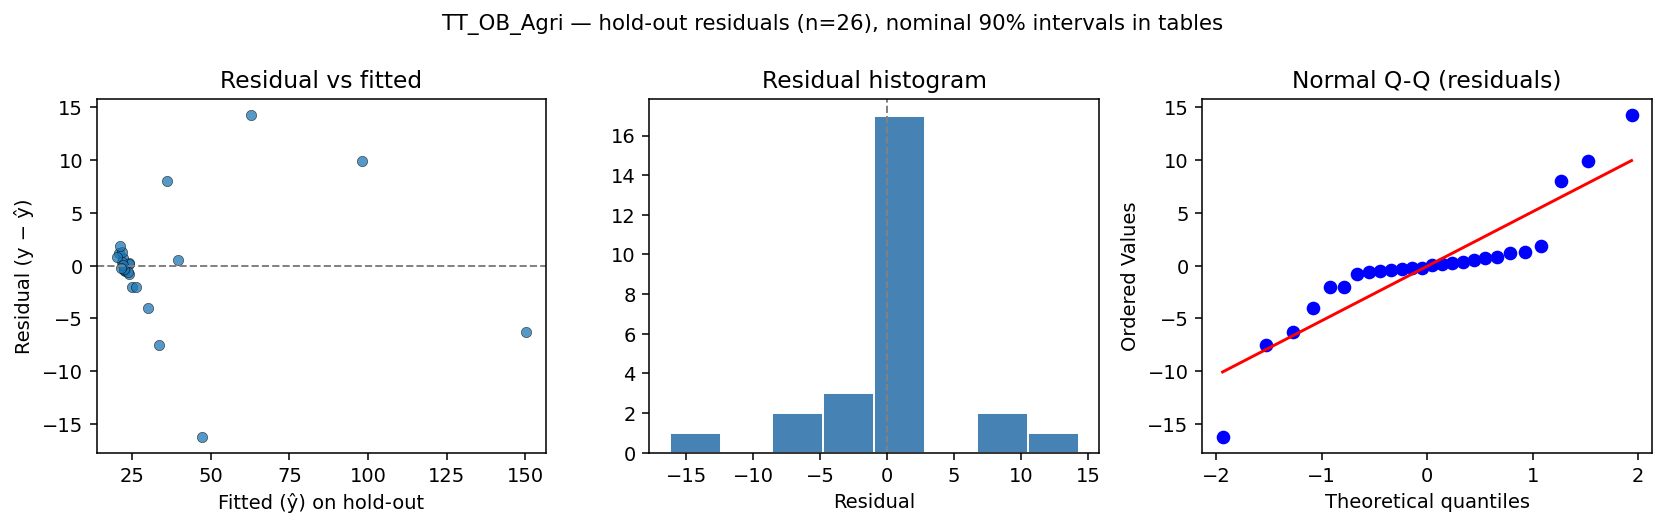
\includegraphics[width=\linewidth]{figures/TT_OB_Agri_holdout_residual_diagnostics.png}
  \caption{\texttt{TT\_OB\_Agri} (ExtraTrees): actual vs.\ predicted hours, residual structure, and count histogram on hold-out ($R^2{=}0.97$).}
  \label{fig:residual-agri}
\end{figure}

\begin{figure}[h]
  \centering
  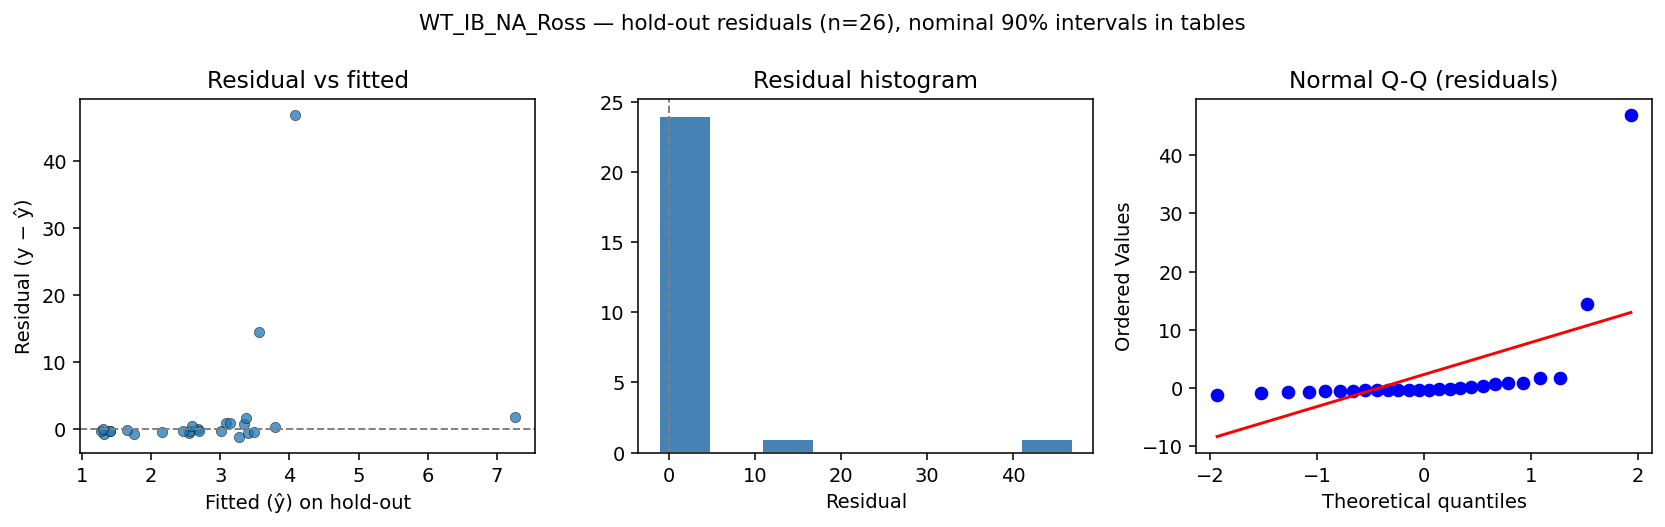
\includegraphics[width=\linewidth]{figures/WT_IB_NA_Ross_holdout_residual_diagnostics.png}
  \caption{\texttt{WT\_IB\_NA\_Ross} (SVR\_RBF): elevated RMSE vs.\ OLS, right-skewed residuals, and systematic bias flag.}
  \label{fig:residual-failure}
\end{figure}

\begin{figure}[h]
  \centering
  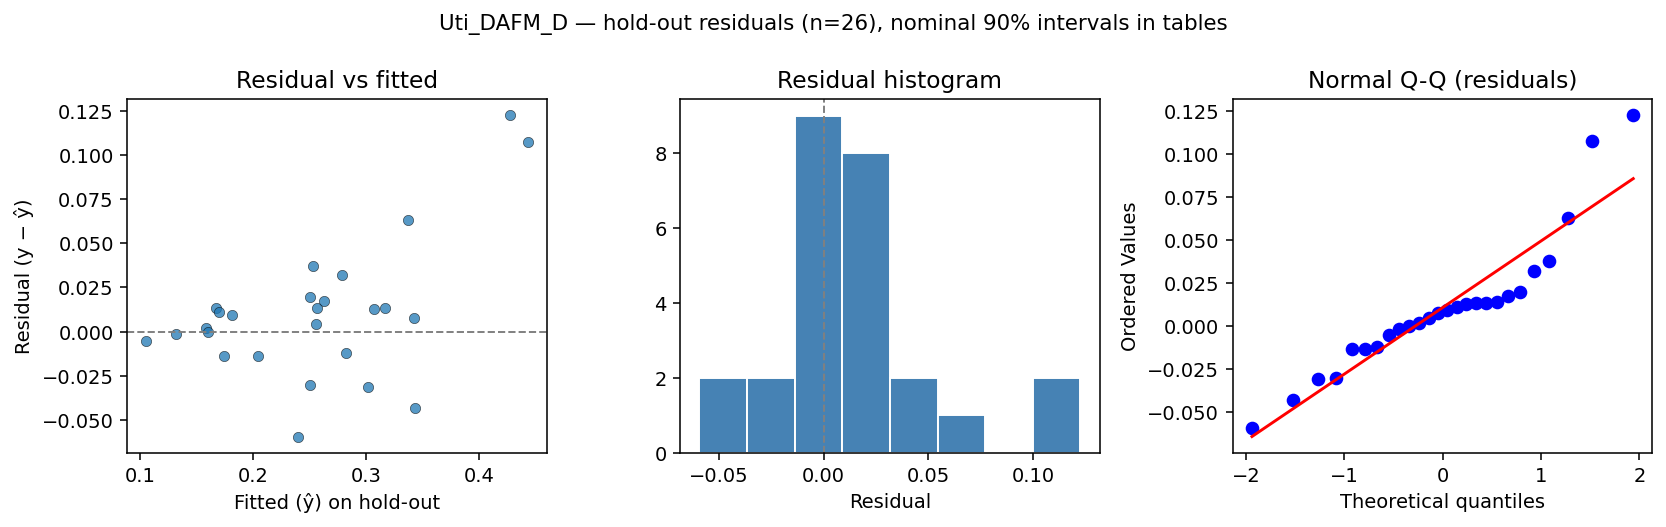
\includegraphics[width=\linewidth]{figures/Uti_DAFM_D_holdout_residual_diagnostics.png}
  \caption{\texttt{Uti\_DAFM\_D} (GPR\_Matern): tight errors on $[0,1]$ utilisation.}
  \label{fig:residual-util}
\end{figure}

\subsection{Model comparison and explainability (placeholders)}

Figure~\ref{fig:heatmap-placeholder} will embed the paired $t$-test $p$-value heatmap (export from \texttt{cv\_fold\_details.xlsx}).

\begin{figure}[h]
  \centering
  \IfFileExists{figures/paired_ttest_pvalue_heatmap.png}{%
    \includegraphics[width=\linewidth]{figures/paired_ttest_pvalue_heatmap.png}}{%
    \fbox{\parbox{0.92\linewidth}{\centering\vspace{1.8cm}\small\textit{Placeholder: paired $t$-test $p$-value heatmap}\\\texttt{figures/paired\_ttest\_pvalue\_heatmap.png}\vspace{1.8cm}}}%
  }
  \caption{Paired $t$-test $p$-values across model pairs (representative target; camera-ready).}
  \label{fig:heatmap-placeholder}
\end{figure}

Figure~\ref{fig:shap-placeholder} will embed a SHAP beeswarm for a representative transit target.

\begin{figure}[h]
  \centering
  \IfFileExists{figures/shap_TT_OB_Agri_beeswarm.png}{%
    \includegraphics[width=\linewidth]{figures/shap_TT_OB_Agri_beeswarm.png}}{%
    \fbox{\parbox{0.92\linewidth}{\centering\vspace{1.8cm}\small\textit{Placeholder: SHAP beeswarm (\texttt{TT\_OB\_Agri})}\\\texttt{figures/shap\_TT\_OB\_Agri\_beeswarm.png}\vspace{1.8cm}}}%
  }
  \caption{Global SHAP beeswarm for \texttt{TT\_OB\_Agri} (\texttt{composite\_pre\_test} winner; camera-ready).}
  \label{fig:shap-placeholder}
\end{figure}

\section{Reproducibility}
\label{app:repro}

From \texttt{experimenting\_ml/}:
\begin{lstlisting}[basicstyle=\ttfamily\footnotesize, breaklines=true]
python run_step1_cv.py --cv-mode repeated10 --n-repeats 3
python run_paired_ttests.py
python run_mentor_step2.py
python run_step3_pre_conformal.py
python run_step6_retrain.py
python run_step4_shap.py --selection composite_pre_test
python run_step7_9_evaluate.py
python run_step10_report.py
python run_ui_inference_api.py
\end{lstlisting}

UI: \url{http://127.0.0.1:8000/UI/index.html}

\section{Group 18 final report extract}
\label{app:group18}

\textbf{Project title (module report):} ML-Driven Web UI for Supply Chain Simulation.
\textbf{Module:} MI6228 Analytics Live.
\textbf{Mentor:} Amr Mahfouz.
\textbf{Team:} Thu Thao Le; Hemant Kumar Ganesen; Inyanila Gnanasekar; Sakshi Jivan Dhamane; Uthara Prarath.

\subsection{Objectives and scope (report \S2)}

\textbf{Measurable objectives:}
(1) near real-time scenario evaluation replacing per-run AnyLogic execution;
(2) hold-out-validated predictive accuracy;
(3) interval-based uncertainty for risk visibility;
(4) SHAP and persona-based attribution in the UI.

\textbf{Scope constraints:} training only on the 129-run NOLHC set (no live port feeds); simulation treated as fixed black box; chatbot limited to in-UI query/response; geography limited to Ireland--GB corridor (Dublin, Rosslare).

\subsection{Architecture layers (report \S4--5)}

Data (NOLHC) $\rightarrow$ ML engine (19 families $\times$ 20 targets, repeated CV, paired $t$-tests, Friedman/Nemenyi) $\rightarrow$ SHAP $\rightarrow$ LLM personas (Executive, Risk, Operations, Analyst) $\rightarrow$ FastAPI $\rightarrow$ web UI.
Post-Brexit inputs span four categories: trade volume shifts, direct-route redistribution, customs/DAFM resources, border-check intervention rates.

\subsection{Validation scenarios (report \S6)}

Example stress cases: 30\% agri SPS physical inspection with elevated customs timings; 25\% landbridge demand shifted via Cherbourg; minimum DAFM bay capacity at both ports.
Decision Intelligence consolidates actual vs.\ predicted (AnyLogic hold-out), RMSE/MAE/$R^2$, interval width/coverage, CV fold stability, and top SHAP features---answering accuracy, certainty, and driver questions in one view.

\subsection{Key findings and limitations (report \S9)}

\textbf{Findings:} surrogates predict all 20 KPIs in real time within acceptable deviation from simulation; UI scenario families cover the four input categories without exposing full model structure; chatbot lowers interpretation barrier.

\textbf{Limitations:} speed--accuracy trade-off and poor extrapolation outside the 129-run envelope; closed-world training (no live freight intelligence; retrain required if simulation ranges change).

\subsection{Appendix artifact index (report)}

\begin{enumerate}
  \item Hyperparameter tuning --- \texttt{cv\_fold\_details.xlsx}
  \item Paired $t$-tests and pipeline summary --- Excel tabs per target
  \item Full experimentation --- \texttt{pipeline\_results.xlsx}, \texttt{experiment\_master.xlsx}
  \item Pre-conformal calibration (top-3 models) --- Step~3 workbook
  \item Conformal intervals --- \texttt{conformal\_results.csv}
  \item SHAP explanations --- \texttt{shap\_master.xlsx}, \texttt{outputs/step4\_shap/}
  \item Parameter groups --- simulation input crosswalk (Appendix~7 in report)
\end{enumerate}

\subsection{Business context (abbreviated)}

\textbf{Value proposition:} avoid AnyLogic Cloud API subscription cost; millisecond predictions; minimalist two-panel UI vs.\ 120+ raw parameters.
\textbf{Stakeholders (Mendelow):} logistics enterprises and data partners (key players); port authorities/regulators (keep satisfied); agri SMEs (keep informed).
\textbf{Go-to-market (conceptual):} Essential / Professional / Enterprise SaaS tiers plus industry pilots and shared scenario library.

\subsection{Figures in PDF report (not embedded here)}

Include in camera-ready if allowed: Figure~4.1 (methodology architecture), Figure~4.2 (training workflow), Figure~5.1 (system architecture), Figure~3.1, SIG presentation slides if separate.

\end{document}